\documentclass[12pt,english]{article}
\usepackage[a4paper,bindingoffset=0.2in,%
            left=0.4in,right=1in,top=1in,bottom=1in,%
            footskip=.25in]{geometry}
\usepackage{amsmath}
\usepackage{amssymb}
\usepackage{graphicx}

\usepackage{listings}
\usepackage{color}
\usepackage{float}

\definecolor{dkgreen}{rgb}{0,0.6,0}
\definecolor{gray}{rgb}{0.5,0.5,0.5}
\definecolor{mauve}{rgb}{0.58,0,0.82}

\lstset{frame=tb,
  language=Matlab,
  aboveskip=3mm,
  belowskip=3mm,
  showstringspaces=false,
  columns=flexible,
  basicstyle={\small\ttfamily},
  numbers=none,
  numberstyle=\tiny\color{gray},
  keywordstyle=\color{blue},
  commentstyle=\color{dkgreen},
  stringstyle=\color{mauve},
  breaklines=true,
  breakatwhitespace=true,
  tabsize=3
}

\graphicspath{ {./grafice/} }

\title{Proiect SCPI\\ Instalatie nivel\\ GB76}
\date{2019\\ Decembrie}
\author{Ionescu Alexandru Cristian - 342 B3\\Pangratie Andrei - 342 B3}

\begin{document}

\maketitle
\newpage

\tableofcontents
\newpage

\section {Etapa 1}
\subsection {Ini}

\begin{table}[H]
  \centering
  \begin{tabular}{|l|l|l|}
    \hline
    GrupID & Comanda nominala $u_0$ & Instalatie \\
    \hline
    GB76 & 55[\%] & nivel \\
    \hline
  \end{tabular}
  \caption{Date initiale}
\end{table}

\subsection {Determinați elementele de execuție si traductoarele}
Poze de pe telefon

\subsection {Care este mărimea fizică care se reglează ?}
A: Inaltimea nominala a lichidului $[m]$

\subsection {Care este mărimea fizică de execuție ?}
A: Debitul de intrare in rezervor $[m^3/s]$

\subsection {Ecuația diferențială care descrie dinamica sistemului}
\begin{center}
  \begin{equation*}
  \rho F_{a}( t) -\rho F_{e}( t) =\dfrac{dM( t)}{dt} =\rho S\dfrac{dL( t)}{dt}
  \end{equation*}
\end{center}

Unde:


\subsection {Care este funcția de transfer echivalentă sistemului ?}
Sistemul poate fi echivalat cu urmatoarea functie de transfer:
\begin{center}
  \begin{equation*}
  H_{p}( s) =\dfrac{K_{p}}{T_{p} s+1}
  \end{equation*}
\end{center}

\subsection {Care sunt parametrii funcției de transfer si cum se pot determina ?}
Parametrii functiei de transfer sunt:
\begin{center}
  \begin{equation*}
  \begin{cases}
  K_{p} & Coeficient\ de\ amplificiare\ al\ sistemului\\
  T_{p} & Constanta\ de\ timp\ specifica\ sistemului
  \end{cases}
  \end{equation*}
\end{center}

Acestia se pot identifica prin mai multe metode:
\begin{enumerate}
  \item Pe cale experimentala, prin analiza raspunsului la treapta
  \item Numeric, prin liniarizarea ecuatiilor diferentiale ce descriu procesul
\end{enumerate}

In continuare, vom explora cea de-a doua metoda:


Se vor liniariza mărimile din sistem după formulele următoare:
\begin{center}
  \begin{equation*}
  \begin{cases}
  L( t) \ =\ L_{0} +\Delta L( t)\\
  F_{a}( t) =F_{a0} +\Delta F_{a}( t)\\
  F_{e}( t) =F_{e0} +\Delta F_{e}( t)
  \end{cases}
  \end{equation*}
\end{center}


\section {Etapa 2}

\subsection {Configurare experiment}

Am pornit WinReg si am comutat intrerupatoarele evidentiate in imagine spre dreapta:

\begin{figure}[H]
  \centering
    \fbox{ 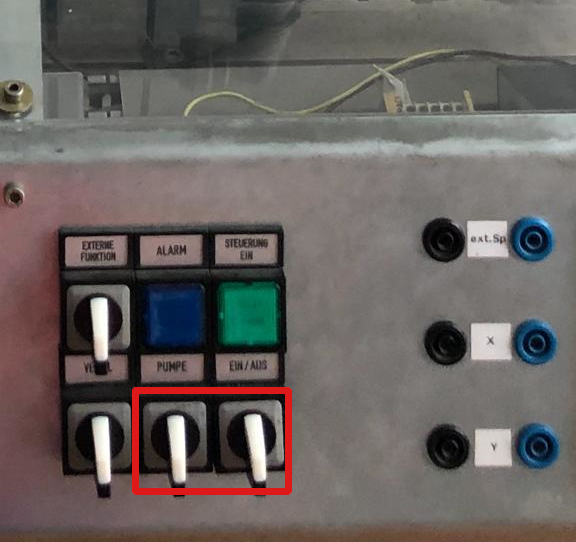
\includegraphics[width=0.8\textwidth]{instalatie_switchuri.png}}
\end{figure}

\subsection {Caracteristici proces}
\begin{table}[H]
  \centering
  \begin{tabular}{|l|l|l|l|}
    \hline
    $t_c$ & $t_t$ & $\tau$ & $T_e\ ales$ \\
    \hline
    123 [s] & 265 [s] & 12 [s] & 1 [s] \\
    \hline
  \end{tabular}
  \caption{Caracteristici proces alese experimental.}
\end{table}

\subsection {Caracteristici proces }

Am aplicat comanda nominala $u_0 = 55\%$, iar dupa am ridicat-o la $u_1 = 75\%$
\begin{figure}[H]
  \centering
    \fbox{ 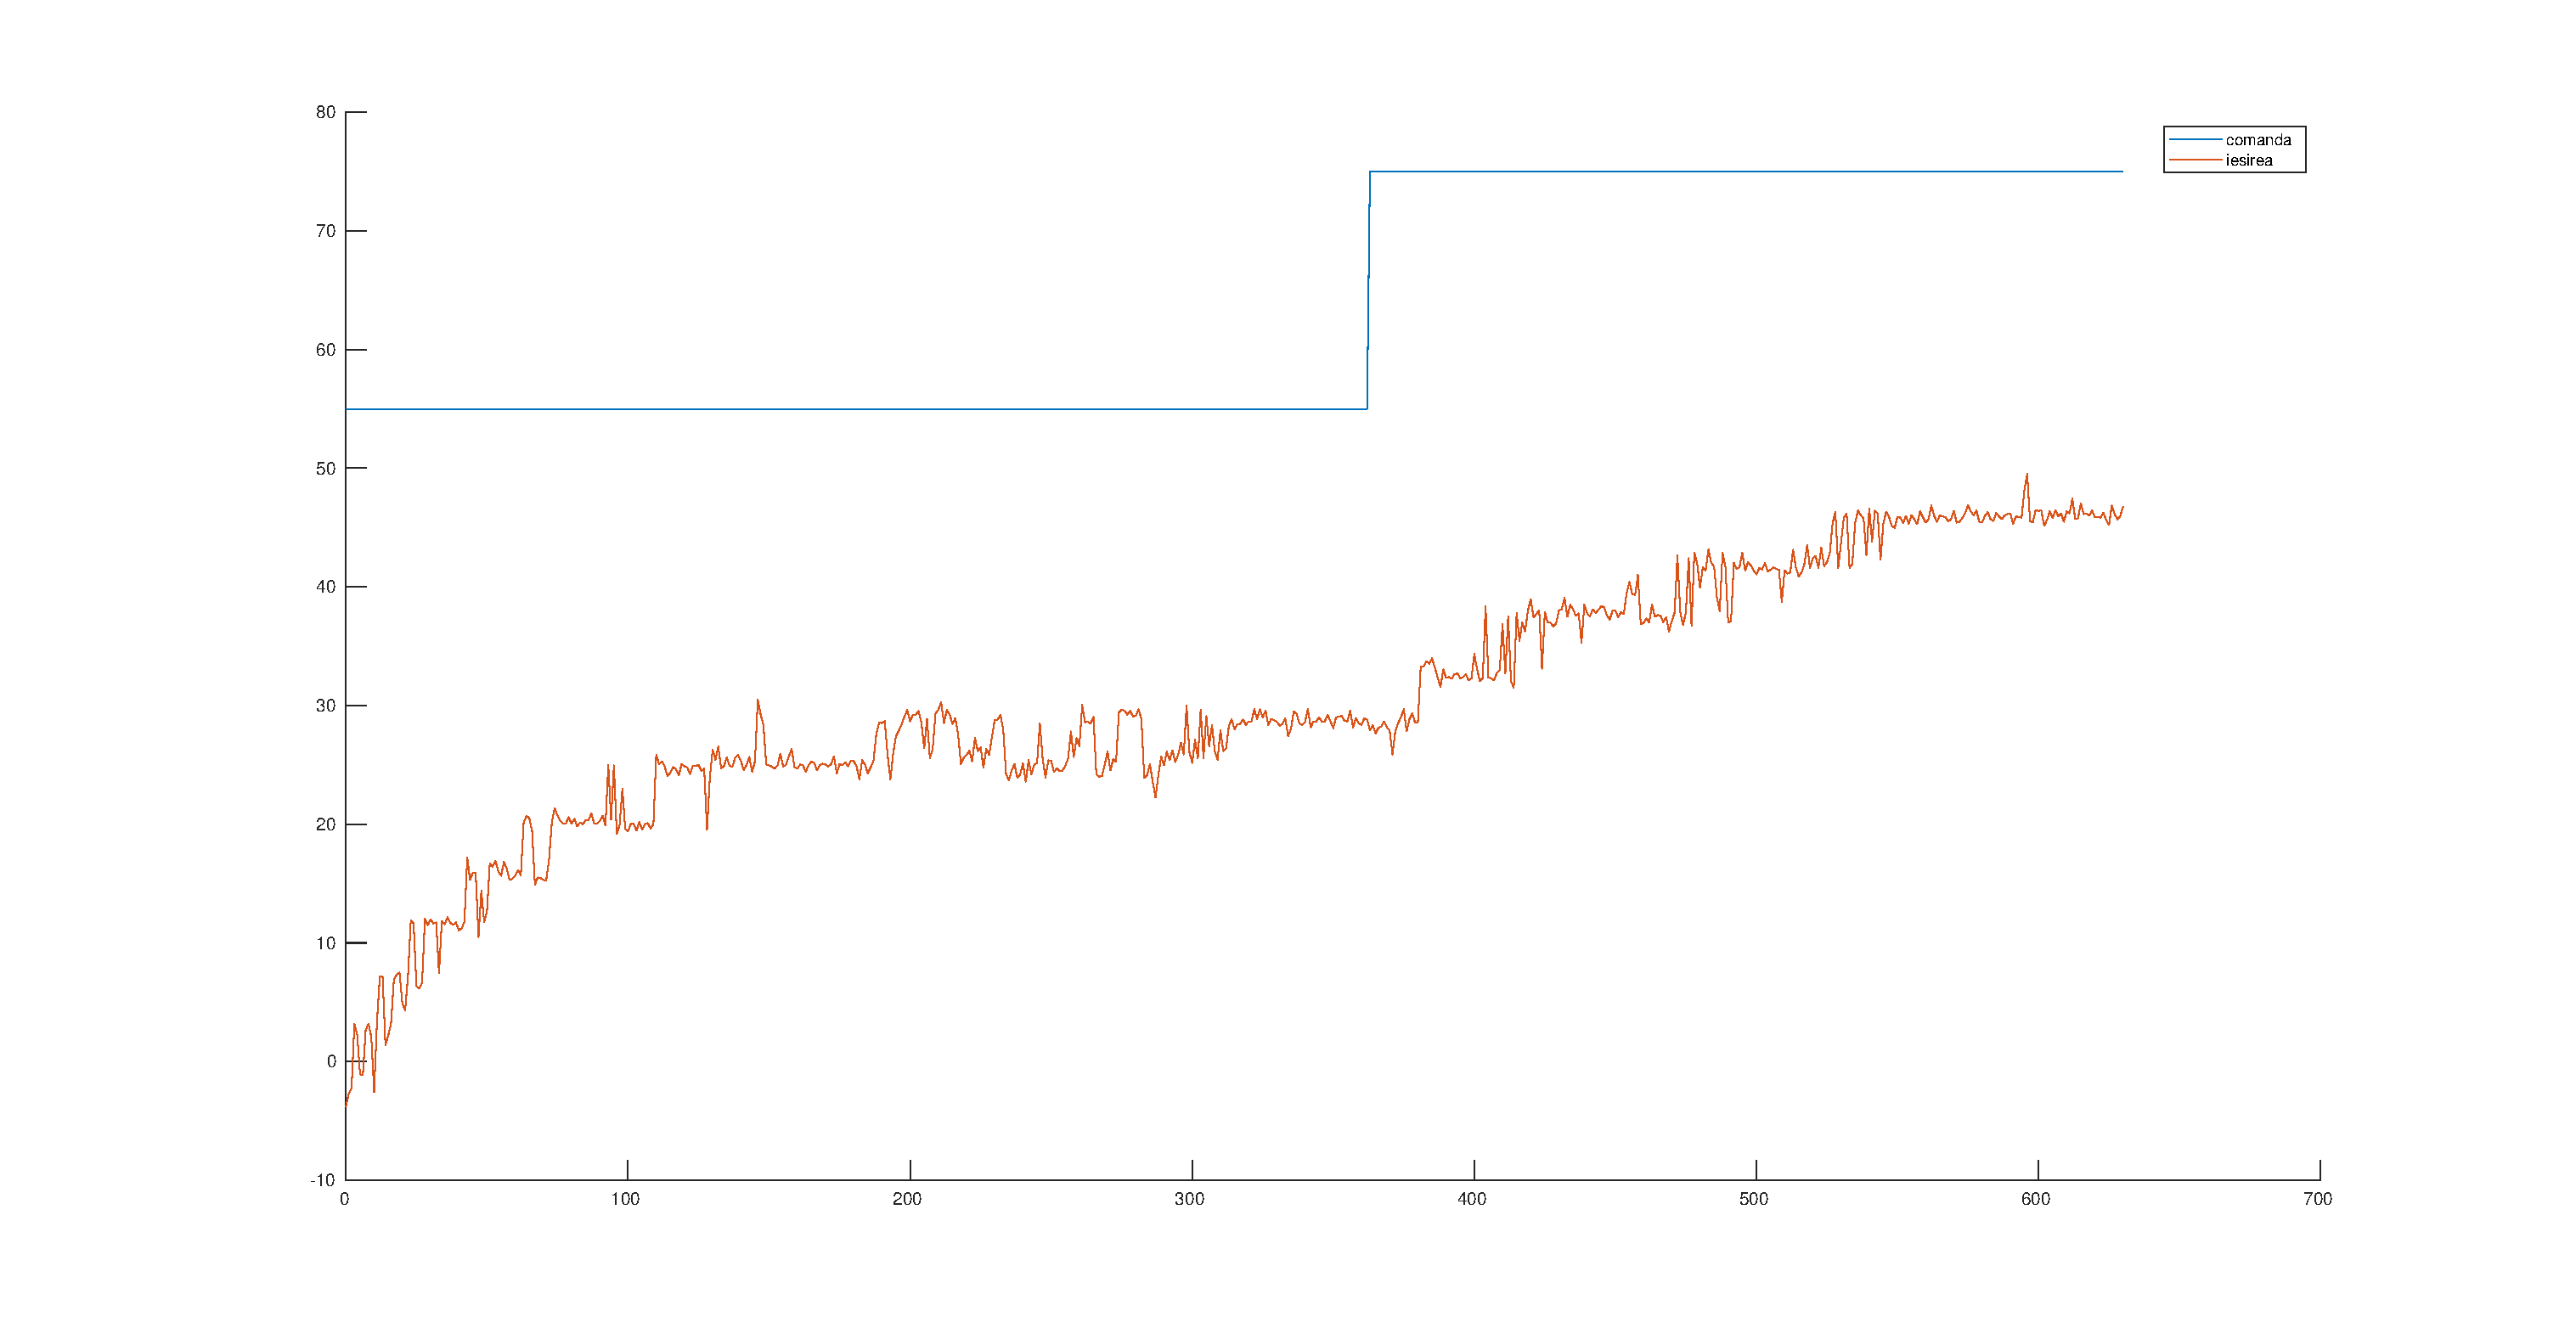
\includegraphics[width=0.8\textwidth]{2_3_1.eps}}
\end{figure}

\subsection {Model liniar}
Pe baza raspunsului la treapta, am propus urmatorul model:
\begin{equation*}
H_{F} =e^{-s\tau }\frac{K_{F}}{T_{F} s+1}
\end{equation*}

unde:
\begin{table}[H]
  \centering
  \begin{tabular}{|l|l|l|l|}
    \hline
    $\tau$ & $K_F$ & $T_F$ & $t_t$ \\
    \hline
    $12 [s]$ & $29/55$ & $160/3$ & $157 [s]$ \\
    \hline
  \end{tabular}
  \caption{Caracteristici model liniarizat.}
\end{table}

Am realizat o simulare a modelului si am suprapus-o peste datele masurate, folosite pentru identificare:

\begin{figure}[H]
  \centering
    \fbox{ 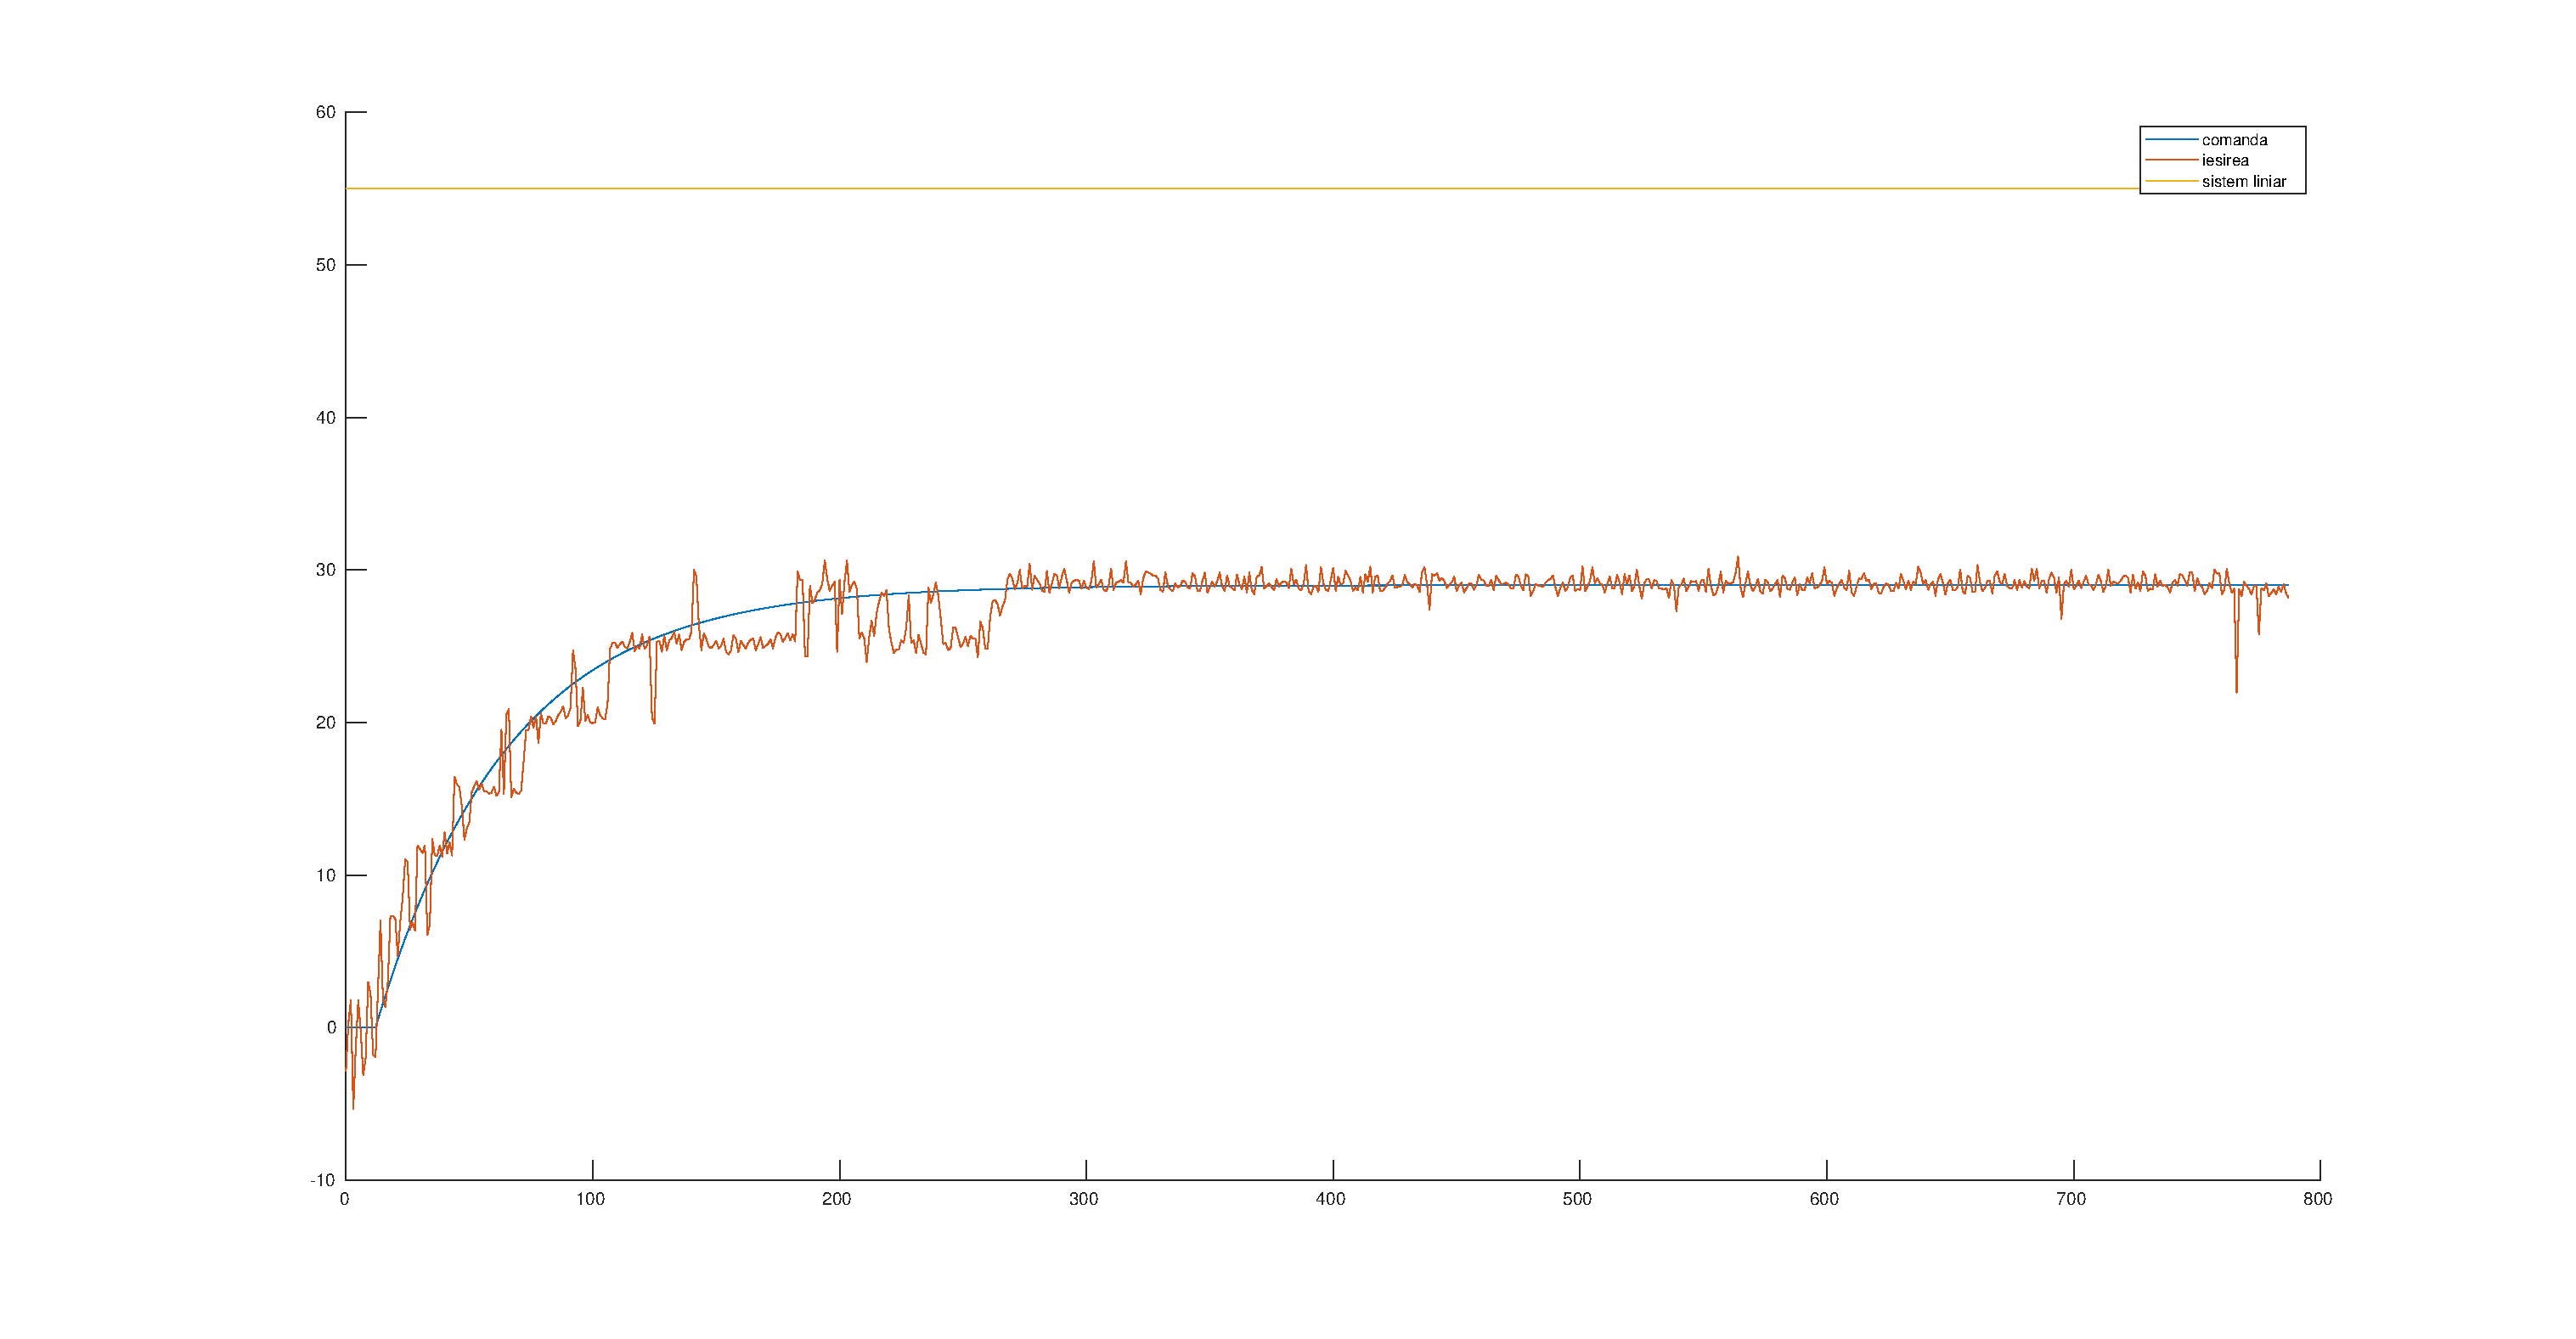
\includegraphics[width=0.8\textwidth]{2_4_1.eps}}
\end{figure}



\section {Etapa 3}



% \begin{center}
%   \fbox{ \includegraphics[width=0.8\textwidth]{8_1_1.eps}}
% \end{center}

\newpage

\subsection {Concluzii}
\begin{itemize}
  \item MCMMPE ofera o precizie inferioara metodei MEMP
  \item Estimarea perturbatiilor oferite de modelul ARX trunchiat duc la pierderea preciziei estimarii
  \item Utila ca baza de initializare in alte problem datorita simplitatii de calcul
\end{itemize}

\section{Cod MATLab}
% \subsection {ISLAB\_6A}
% \lstinputlisting[firstline=174,lastline=387]{../Scripts/ISLAB_6A.m}

\end{document}